\documentclass{beamer}
\usepackage[utf8]{inputenc}
\usepackage[english]{babel}
\usepackage{helvet}
\usepackage[T1]{fontenc}
\usepackage[inline]{asymptote}
\usepackage{asy_helper}
\usepackage{slide_helper}
\usepackage{multirow}
\usepackage{cancel}
\usepackage{tikz}
\usetikzlibrary{shapes.geometric, arrows}
\usepackage{pgfplots}
\pgfplotsset{compat=1.5} 
\usepgfplotslibrary{statistics}
\usetikzlibrary{external}
\tikzexternalize%

\begin{asydef}
  import gsl;
  
  real nd_func(real mu, real sigma, real x)
  {
    return 1/sqrt(2*pi*sigma*sigma)*exp((-1*(x-mu)*(x-mu))/(2*sigma*sigma));
  }
  
  guide normal_dist(real mu, real sigma, real xmin, real xmax)
  {
    real nd(real x) { return nd_func(mu, sigma, x); }
    return graph(nd, xmin, xmax);
  }

  guide t_dist(real df, real xmin, real xmax)
  {
    real f(real x) { return pdf_tdist(x, df); }
    return graph(f, xmin, xmax);
  }

  void shade_below(real mu, real sigma, real b, real xmin, real xmax, pen p=royalblue)
  {
    real nd_func(real x) { return 1/sqrt(2*pi*sigma*sigma)*exp((-1*(x-mu)*(x-mu))/(2*sigma*sigma)); }
    
    guide g = graph(nd_func, xmin, b);
    
    filldraw(g -- (b,0) -- cycle, p, black);
    
    draw((xmin,0)--(b,0));
  }

  void shade_above(real mu, real sigma, real b, real xmin, real xmax, pen p=royalblue)
  {
    real nd_func(real x) { return 1/sqrt(2*pi*sigma*sigma)*exp((-1*(x-mu)*(x-mu))/(2*sigma*sigma)); }
    
    guide g = graph(nd_func, b, xmax);
    
    filldraw(g -- (b,0) -- cycle, p, black);
    
    draw((xmax,0)--(b,0));
  }

  void shade_between(real mu, real sigma, real a, real b, pen p=royalblue)
  {
    real nd_func(real x) { return 1/sqrt(2*pi*sigma*sigma)*exp((-1*(x-mu)*(x-mu))/(2*sigma*sigma)); }
    
    guide g = graph(nd_func, a, b);
    
    filldraw((a,0) -- g -- (b,0) -- cycle, p, black);
  }

  void multiple_nd_curves_example(real std_dev)
  {
    size(300, 190, IgnoreAspect);
    
    draw(normal_dist(0, std_dev, -6,6));
    shade_between(0,std_dev,-std_dev,std_dev);
    draw((0,0)--(0,0.45));

    label("$\sigma="+format("%#.2f", std_dev)+"$", (-4.2,0.45), Fill(paleyellow));

    xaxis(Bottom(), RightTicks(new real[] {-6,-4,-2,0,2,4,6}));
    yaxis(Left(), LeftTicks(size=nan),ymin = 0, ymax = 0.5);
  }
\end{asydef}

\newcommand{\satisfied}[0]{{\color{green!70!black}\checkmark}}

\title[MA205 - Section 7.1]{One-sample means with the $t$-distribution}

\newcommand{\prob}[1]{P\left({#1}\right)}
\newcommand{\jointprob}[3]{\prob{{#1}~\text{#2}~{#3}}}
\newcommand{\condprob}[2]{\prob{{#1}~|~{#2}}}
\newcommand{\comb}[2]{_{#1}C_{#2}}

\begin{document}
\begin{frame}
  \titlepage
\end{frame}

\begin{frame}
  \begin{block}{Central Limit Theorem for the Sample Mean}
    When we collect a sufficiently large sample of $n$ independent observations from a population with mean $\mu$ and standard deviation $\sigma$, the sampling distribution of $\bar{x}$ will be nearly normal with:
    \begin{equation*}
      \begin{aligned}
        \text{Mean} = \mu
        \qquad\qquad
        \text{Standard Deviation ($SE$)} = \dfrac{\sigma}{\sqrt{n}}
      \end{aligned}
    \end{equation*}
  \end{block}\pause

  \begin{note}
    It's rare to need to estimate the population mean $\mu$, but somehow know the population standard deviation $\sigma$. In most cases $\sigma$ will need to be estimated.
  \end{note}
\end{frame}

\begin{frame}
  \begin{block}{Conditions to Apply the Central Limit Theorem}
    \begin{description}
    \item[Independence:] The sample observations must be independent.\pause
    \item[Normality:] When a sample is small, we also require that the sample observations come from a normally distributed population.\pause
      \begin{description}
      \item[$\boldsymbol{n<30}$:] If the sample size $n$ is less than 30 and there are no clear outliers in the data, then we typically assume the data is from a nearly normal population.\pause
      \item[$\boldsymbol{n\geq30}$:] If the sample size $n$ is at least 30 and there are no \emph{particularly extreme outliers}, then we typically assume the sampling distribution of $\bar{x}$ is nearly normal, even if the underlying population is not.
      \end{description}
    \end{description}
  \end{block}\pause
  
  \begin{note}
    In a first course in statistics, you aren't expected to develop perfect judgment on the normality condition.
  \end{note}
\end{frame}

\begin{frame}
  \begin{example}
    \begin{center}
      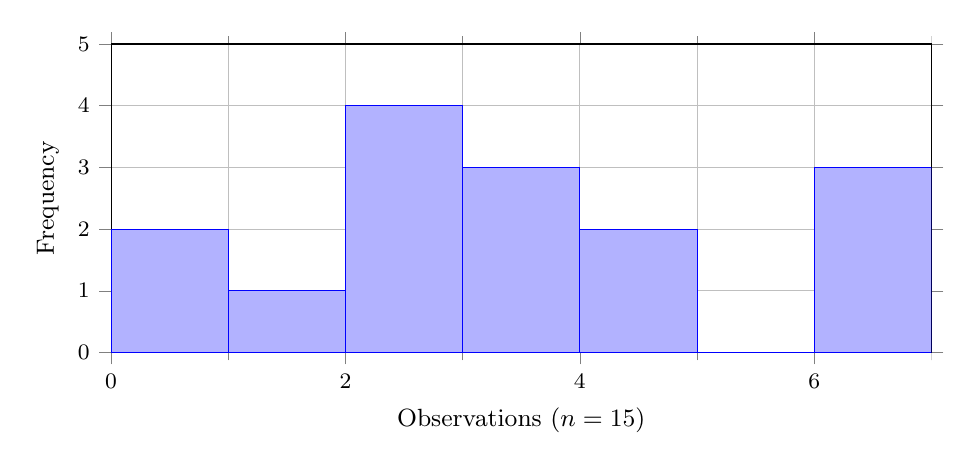
\begin{tikzpicture}
        \begin{axis}[
            small,
            height=5.5cm,
            width=12.0cm,
            enlarge x limits=false,
            enlarge y limits=false,
            %ybar interval,
            grid=both,
            %minor y tick num=1,
            minor x tick num=1,
            ylabel={Frequency},
            xlabel={Observations ($n=15$)},
            %x tick label style={rotate=0,anchor=south east},
            tick align=outside, % <-- this positions the ticks "outside"
            xtick={0, 2, 4,...,30},
            ytick={0, 1,...,30},
            ymin=0,
            ymax=5,
            xmin=0,
            xmax=7,
            xticklabel style={/pgf/number format/.cd,fixed,precision=0},
            xticklabel=
            \pgfmathprintnumber\tick,%--\pgfmathprintnumber\nexttick\%,
          ]
          \draw [blue,fill=blue!30!white] (axis cs: 0,0) rectangle (axis cs: 1,2);
          \draw [blue,fill=blue!30!white] (axis cs: 1,0) rectangle (axis cs: 2,1);
          \draw [blue,fill=blue!30!white] (axis cs: 2,0) rectangle (axis cs: 3,4);
          \draw [blue,fill=blue!30!white] (axis cs: 3,0) rectangle (axis cs: 4,3);
          \draw [blue,fill=blue!30!white] (axis cs: 4,0) rectangle (axis cs: 5,2);
          \draw [blue,fill=blue!30!white] (axis cs: 5,0) rectangle (axis cs: 6,0);
          \draw [blue,fill=blue!30!white] (axis cs: 6,0) rectangle (axis cs: 7,3);
        \end{axis}
      \end{tikzpicture}
    \end{center}

    \vspace{-4mm}
    \question{Is the normality condition met?}\pause
    \answer{Since there are less than 30 observations, we need to look for \emph{clear} outliers. While there is a gap on the right, the gap is small and 20\% of the observations fall in rightmost bar. We can't really call these clear outliers, so the normality condition is reasonably met.}
  \end{example}
\end{frame}

\begin{frame}
  \begin{example}
    \begin{center}
      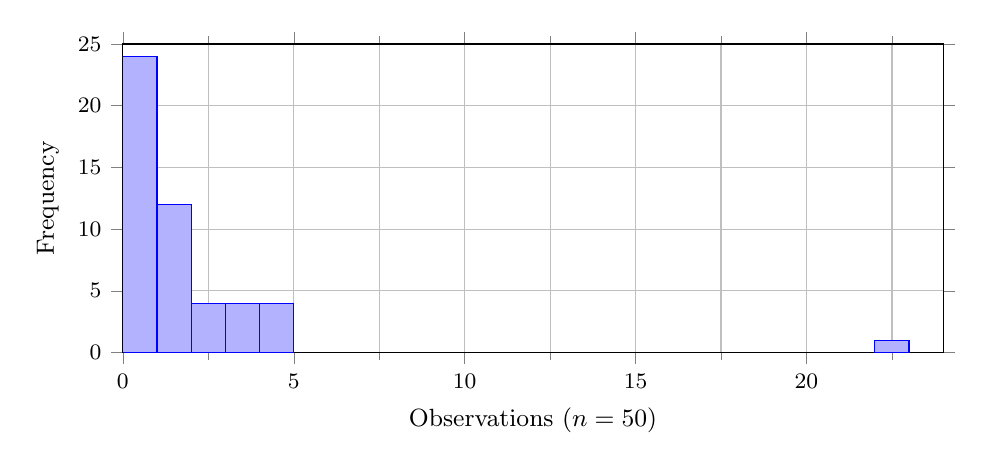
\begin{tikzpicture}
        \begin{axis}[
            small,
            height=5.5cm,
            width=12.0cm,
            enlarge x limits=false,
            enlarge y limits=false,
            %ybar interval,
            grid=both,
            %minor y tick num=1,
            minor x tick num=1,
            ylabel={Frequency},
            xlabel={Observations ($n=50$)},
            %x tick label style={rotate=0,anchor=south east},
            tick align=outside, % <-- this positions the ticks "outside"
            xtick={0, 5, 10,...,30},
            ytick={0, 5,...,30},
            ymin=0,
            ymax=25,
            xmin=0,
            xmax=24,
            xticklabel style={/pgf/number format/.cd,fixed,precision=0},
            xticklabel=
            \pgfmathprintnumber\tick,%--\pgfmathprintnumber\nexttick\%,
          ]
          \draw [blue,fill=blue!30!white] (axis cs: 0,0) rectangle (axis cs: 1,24);
          \draw [blue,fill=blue!30!white] (axis cs: 1,0) rectangle (axis cs: 2,12);
          \draw [blue,fill=blue!30!white] (axis cs: 2,0) rectangle (axis cs: 3,4);
          \draw [blue,fill=blue!30!white] (axis cs: 3,0) rectangle (axis cs: 4,4);
          \draw [blue,fill=blue!30!white] (axis cs: 4,0) rectangle (axis cs: 5,4);
          \draw [blue,fill=blue!30!white] (axis cs: 22,0) rectangle (axis cs: 23,1);
        \end{axis}
      \end{tikzpicture}
    \end{center}

    \vspace{-4mm}
    \question{Is the normality condition met?}\pause
    \answer{The sample size is greater than 30, so we need to look for an extreme outlier. The gap is more than four times the width of the cluster on the left side, so this is clearly an extreme outlier and the normality condition is not met.}
  \end{example}
\end{frame}

\begin{frame}
  \begin{note}
    In practice, we cannot directly calculate the standard error for $\bar{x}$, since we do not know the population standard deviation $\sigma$.\pause

    \vspace{1mm}
    We can use the sample standard deviation $s$ as the best estimate of $\sigma$:

    \vspace{-2mm}
    \begin{equation*}
      \begin{aligned}
        SE = \dfrac{\sigma}{\sqrt{n}}\approx\dfrac{s}{\sqrt{n}}
      \end{aligned}
    \end{equation*}
  \end{note}\pause
  
  \begin{definition}
    If a population has a normal distribution, then the distribution of 
    \begin{equation*}
      t = \dfrac{\bar{x}-\mu}{SE} \approx \dfrac{ \bar{x}-\mu }{ \dfrac{s}{ \sqrt{n} } }
    \end{equation*}
    is called the \textbf{Student $\boldsymbol{t}$ distribution} for sample sizes $n$.
  \end{definition}\pause

  \begin{note}
    A Student $t$ distribution is commonly called a \textbf{$\boldsymbol{t}$ distribution}.
  \end{note}
\end{frame}

\begin{frame}
  \begin{definition}
    The \textbf{degrees of freedom} (or \textbf{df}) for a collection of sample data is the number of sample values that can vary after certain restrictions have been imposed on all data values.

    \vspace{1mm}
    When modeling $\bar{x}$ using the $t$-distribution, use:

    \vspace{-4mm}
    \begin{equation*}
      df = n-1
    \end{equation*}
  \end{definition}\pause

  \begin{example}
    If 10 test scores must have mean 80, then their sum must be 800.\pause

    \vspace{2mm}
    We can freely assign values to the first 9 scores, but the 10th score would need to be:

    \vspace{-4mm}
    \begin{equation*}
      \text{s}_{10} = 800 - \text{s}_1 - \text{s}_2 - \text{s}_3 - \text{s}_4 - \text{s}_5 - \text{s}_6 - \text{s}_7 - \text{s}_8 - \text{s}_9
    \end{equation*}\pause

    \vspace{-4mm}
    Hence 9 degrees of freedom.
  \end{example}
\end{frame}

\begin{frame}[fragile]
  \begin{note}
    The Student $t$ distribution changes for different degrees of freedom.

    \vspace{1mm}
    \begin{overprint}
      \onslide<1 | handout:0>
      \begin{center}
        \begin{asy}
          size(200,95, IgnoreAspect);

          real xmin = -3.5; real xmax = 3.5;

          draw(normal_dist(0,1,xmin,xmax), black+dashed, "Std Normal");

          draw(t_dist(8, xmin, xmax), invisible, "$\phantom{df=8}$");
          draw(t_dist(4, xmin, xmax), invisible, "$\phantom{df=4}$");
          draw(t_dist(2, xmin, xmax), invisible, "$\phantom{df=2}$");
          draw(t_dist(1, xmin, xmax), invisible, "$\phantom{df=1}$");

          xaxis(Ticks(new real[] {0}));

          attach(legend(), truepoint(E), 10E, UnFill);
        \end{asy}
      \end{center}
      \onslide<2 | handout:0>
      \begin{center}
        \begin{asy}
          size(200,95, IgnoreAspect);

          real xmin = -3.5; real xmax = 3.5;

          draw(normal_dist(0,1,xmin,xmax), black+dashed, "Std Normal");

          draw(t_dist(8, xmin, xmax), invisible, "$\phantom{df=8}$");
          draw(t_dist(4, xmin, xmax), invisible, "$\phantom{df=4}$");
          draw(t_dist(2, xmin, xmax), invisible, "$\phantom{df=2}$");
          draw(t_dist(1, xmin, xmax), palered, "$df=1$");
          
          xaxis(Ticks(new real[] {0}));

          attach(legend(), truepoint(E), 10E, UnFill);
        \end{asy}
      \end{center}
      \onslide<3 | handout:0>
      \begin{center}
        \begin{asy}
          size(200,95, IgnoreAspect);

          real xmin = -3.5; real xmax = 3.5;

          draw(normal_dist(0,1,xmin,xmax), black+dashed, "Std Normal");

          draw(t_dist(8, xmin, xmax), invisible, "$\phantom{df=8}$");
          draw(t_dist(4, xmin, xmax), invisible, "$\phantom{df=4}$");
          draw(t_dist(2, xmin, xmax), lightred, "$df=2$");
          draw(t_dist(1, xmin, xmax), palered, "$df=1$");

          xaxis(Ticks(new real[] {0}));

          attach(legend(), truepoint(E), 10E, UnFill);
        \end{asy}
      \end{center}
      \onslide<4 | handout:0>
      \begin{center}
        \begin{asy}
          size(200,95, IgnoreAspect);

          real xmin = -3.5; real xmax = 3.5;

          draw(normal_dist(0,1,xmin,xmax), black+dashed, "Std Normal");

          draw(t_dist(8, xmin, xmax), invisible, "$\phantom{df=8}$");
          draw(t_dist(4, xmin, xmax), red, "$df=4$");
          draw(t_dist(2, xmin, xmax), lightred, "$df=2$");
          draw(t_dist(1, xmin, xmax), palered, "$df=1$");
                
          xaxis(Ticks(new real[] {0}));

          attach(legend(), truepoint(E), 10E, UnFill);
        \end{asy}
      \end{center}
      \onslide<5- | handout:1>
      \begin{center}
        \begin{asy}
          size(200,95, IgnoreAspect);

          real xmin = -3.5; real xmax = 3.5;

          draw(normal_dist(0,1,xmin,xmax), black+dashed, "Std Normal");

          draw(t_dist(8, xmin, xmax), heavyred, "$df=8$");
          draw(t_dist(4, xmin, xmax), red, "$df=4$");
          draw(t_dist(2, xmin, xmax), lightred, "$df=2$");
          draw(t_dist(1, xmin, xmax), palered, "$df=1$");
          
          xaxis(Ticks(new real[] {0}));

          attach(legend(), truepoint(E), 10E, UnFill);
        \end{asy}
      \end{center}
    \end{overprint}
  \end{note}

  \onslide<6->
  \begin{note}
    The $t$-distribution has a mean of $t=0$ 

    \vspace{1mm}
    The standard deviation varies with $n$, but is always greater than 1.
  \end{note}

  \onslide<7->
  \begin{note}
    As the sample size gets larger, the Student $t$ distribution gets closer to the standard normal distribution.
  \end{note}
\end{frame}

%% \begin{frame}[fragile]
%%   \begin{example}
%%     Let us find the critical value corresponding to a 95\% confidence level, given that the sample size is $n=15$.\pause

%%     \vspace{2mm}
%%     The degrees of freedom is $n-1=15-1=14$.\pause

%%     \vspace{2mm}
%%     We can then use technology to find the critical value.

%%     \begin{center}
%%       \begin{asy}
%%         size(200,100, IgnoreAspect);

%%         real xmin = -3.5; real xmax = 3.5;

%%         real a = -2.145;
%%         real b = 2.145;

%%         guide g = t_dist(14, xmin, a);
%%         filldraw((xmin,0) -- g -- (a,0) -- cycle, orange, black);
%%         guide g = t_dist(14, b, xmax);
%%         filldraw((b,0) -- g -- (xmax,0) -- cycle, orange, black);
%%         guide g = t_dist(14, a, b);
%%         filldraw((a,0) -- g -- (b,0) -- cycle, yellow, black);
%%         draw(t_dist(14, xmin, xmax), black);

%%         label("0.95", (0, 0.5*pdf_tdist(0,14)));
%%         label("0.025", (a, pdf_tdist(a,14)), 3W);
%%         label("0.025", (b, pdf_tdist(b,14)), 3E);

%%         draw_tick("$t=0$", (0,0));
%%         draw_tick("$t_{\alpha/2}=2.145$", (2.145,0));

%%         xaxis();

%%         attach(legend(), truepoint(E), 10E, UnFill);
%%       \end{asy}
%%     \end{center}
%%   \end{example}
%% \end{frame}

%% \begin{frame}
%%   \begin{block}{Procedure for Constructing a Confidence Interval for $\mu$}
%%     \begin{enumerate}[<+- | alert@+>]
%%     \item Verify that the following requirements are satisfied:
%%       \begin{itemize}
%%       \item<.-> The sample is a simple random sample.
%%       \item<.-> Population is normally distributed or $n>30$.
%%       \end{itemize}
%%     \item Use technology to find the critical value $t_{\alpha/2}$.
%%       \begin{itemize}
%%       \item<.-> When $\sigma$ is unknown, use $n-1$ degrees of freedom.
%%       \end{itemize}
%%     \item Calculate the margin of error.
%%       \begin{equation*}
%%         E=t_{\alpha/2}\cdot\dfrac{s}{\sqrt{n}}
%%       \end{equation*}
%%     \item Using the value of the calculated margin of error $E$ and the value of the sample mean $\bar{x}$, find the values of the confidence interval limits $\bar{x}-E$ and $\bar{x}+E$.
%%     \item Round the resulting confidence interval limits:
%%       \begin{itemize}
%%       \item<.-> With an original data set, round to three significant digits.
%%       \item<.-> When using summary statistics, round to the same number of decimal places.
%%       \end{itemize}
%%     \end{enumerate}
%%   \end{block}
%% \end{frame}

%% \begin{frame}
%%   \begin{example}
%%     The weights (in hectograms, hg) of randomly selected girls at birth are

%%     \vspace{-7mm}
%%     \begin{center}
%%       \begin{tabular}{ccccccccccccccc}
%%         33 & 28 & 33 & 37 & 31 & 32 & 31 & 28 & 34 & 28 & 33 & 26 & 30 & 31 & 28
%%       \end{tabular}
%%     \end{center}

%%     \vspace{-3mm}
%%     (Based on data from the National Center for Health Statistics.)\pause

%%     \vspace{1mm}
%%     The summary statistics for this sample are
%%     \vspace{-2mm}
%%     \begin{equation*}
%%       n = 15
%%       \qquad\qquad \bar{x} = 30.9
%%       \qquad\qquad s  = 2.9
%%     \end{equation*}\pause

%%     \vspace{-7mm}
%%     Let's construct a 95\% confidence interval for the mean birth weight of girls.\pause

%%     \vspace{1mm}
%%     The margin of error is

%%     \vspace{-3mm}
%%     \begin{equation*}
%%       E=t_{\alpha/2}\cdot\dfrac{s}{\sqrt{n}}\pause
%%       =2.145\cdot\dfrac{2.9}{\sqrt{15}}\pause
%%       =1.606126
%%     \end{equation*}\pause

%%     \vspace{-4mm}
%%     The confidence interval is

%%     \vspace{-3mm}
%%     \begin{equation*}
%%       \begin{matrix}
%%         \bar{x} - E &<& \mu &<& \bar{x} + E\\\pause
%%         30.9 - 1.606126 &<& \mu &<& 30.9 + 1.606126 \\\pause
%%         29.3~\text{hg} &<& \mu &<& 32.5~\text{hg} \\
%%       \end{matrix}
%%     \end{equation*}\pause

%%     \vspace{-3mm}
%%     We are 95\% confident that the interval from 29.2 hg to 32.5 hg actually does contain the true value of $\mu$.
%%   \end{example}
%% \end{frame}

%% \begin{frame}
%%   \begin{block}{Finding $\bar{x}$ from a Confidence Interval}
%%     If you know the confidence interval limits, we can calculate the point estimate:
%%     \begin{equation*}
%%       \bar{x} = \dfrac{(\text{upper confidence interval limit})+(\text{lower confidence interval limit})}{2}
%%     \end{equation*}
%%   \end{block}\pause

%%   \begin{block}{Finding $E$ from a Confidence Interval}
%%     If you know the confidence interval limits, we can calculate the margin of error:
%%     \begin{equation*}
%%       E = \dfrac{(\text{upper confidence interval limit})-(\text{lower confidence interval limit})}{2}
%%     \end{equation*}
%%   \end{block}
%% \end{frame}

%% \begin{frame}[fragile]
%%   \begin{example}
%%     We can compare the confidence intervals of the mean cotinine level in each of three samples (Data Set 12).
%%     \begin{center}
%%       \begin{asy}
%%         size(200,60, IgnoreAspect);

%%         void draw_CI(real l, real r, real h, pen p)
%%         {
%% 	  draw((l,h) -- (r,h), p+1bp);
%% 	  dot((l,h), p);
%% 	  dot((r,h), p);
%%         }

%%         draw_CI(0, 40, 1, blue);
%%         label("People not exposed to smoke", (40,1), E);
%%         draw_CI(25, 110, 2, red);
%%         label("People exposed to smoke", (110,2), E);
%%         draw_CI(140, 220, 3, yellow);
%%         label("Smokers", (140,3), W);

%%         draw((-25,0)--(225,0));
%%         for(real i=-25; i<=225; i +=25)
%% 	draw_tick(string(i),(i,0),.1);
%%       \end{asy}
%%     \end{center}
%%     Because cotinine is produced in the body when nicotine is absorbed, cotinine is a good indication of nicotine intake.\pause

%%     \vspace{2mm}
%%     We see that the confidence interval for smokers does not overlap the other confidence intervals, so it appears that the mean cotinine level of smokers is different from that of the other two groups.\pause

%%     \vspace{2mm}
%%     The two non-smoking groups have overlapping confidence intervals, so it possible that they have the same mean cotinine level.
%%   \end{example}
%% \end{frame}

%% \begin{frame}
%%   \begin{block}{Caution}
%%     Confidence intervals can be used to \emph{informally} compare different data sets, but the overlapping of confidence intervals \emph{should not } be used for making formal and final conclusions about equality of means.
%%   \end{block}\pause

%%   \begin{block}{Sample Size Required to Estimate a Population Mean}
%%     The sample must be a simple random sample of independent sample units.\pause

%%     \vspace{2mm}
%%     We must know, or have estimated, the population standard deviation $\sigma$.\pause

%%     \vspace{2mm}
%%     The required sample size is

%%     \vspace{-2mm}
%%     \begin{equation*}
%%       n={\left(\dfrac{z_{\alpha/2}\cdot\sigma}{E}\right)}^2
%%     \end{equation*}
%%     (Recall that $z_{\alpha/2}$ is the critical value for the standard normal distribution.)
%%   \end{block}\pause

%%   \begin{block}{Rounding}
%%     If the computed sample size $n$ is not a whole number, round the value of $n$ up to the next larger whole number.
%%   \end{block}
%% \end{frame}

%% \begin{frame}
%%   \begin{block}{Dealing with Unknown $\sigma$ When Finding Sample Size}
%%     \begin{enumerate}[<+- | alert@+>]
%%     \item Use the range rule of thumb:
%%       \begin{equation*}
%%         \sigma\approx \text{range}/4
%%       \end{equation*}
%%     \item Start the sample collection process without knowing $\sigma$ and, using the first several values, calculate the sample standard deviation $s$ and use it in place of $\sigma$.
%%       \begin{itemize}
%%       \item The estimate for $\sigma$ can be improved as more sample data are collected, and the required sample size can be adjusted along the way.
%%       \end{itemize}
%%     \item Estimate the value of $\sigma$ by using the results of some other earlier study.
%%     \end{enumerate}
%%   \end{block}

%%   \onslide<+->
%%   \begin{block}{Caution}
%%     When determining the sample size $n$, any errors should always be conservative in the sense that they make the sample size too large instead of too small.
%%   \end{block}
%% \end{frame}

%% \begin{frame}
%%   \begin{example}
%%     Suppose that we want the mean IQ for the population of all Colby students. \pause

%%     \vspace{1mm}
%%     How many Colby students must be randomly selected for IQ tests if we want 95\% confidence that the sample mean is within 3 IQ points of the population mean?\pause

%%     \vspace{1mm}
%%     For a 95\% confidence interval, we have $\alpha=0.5$, so $z_{\alpha/2}=1.96$. \pause

%%     \vspace{1mm}
%%     Our desired margin of error is $E=3$.\pause

%%     \vspace{1mm}
%%     Wechsler IQ tests are designed so that the standard deviation is 15.\pause

%%     \vspace{1mm} 
%%     While we don't know the $\sigma$ of all Colby students, we can safely assume that they are a more homogeneous group than the general population, and hence have a standard deviation less than 15. Thus, we can use $\sigma=15$.\pause

%%     Using the formula for sample size we get
%%     \vspace{-1mm}
%%     \begin{equation*}
%%       n={\left(\dfrac{z_{\alpha/2}\cdot\sigma}{E}\right)}^2\pause
%%       ={\left(\dfrac{1.96\cdot 15}{3}\right)}^2\pause
%%       = 96.04
%%     \end{equation*}\pause

%%     \vspace{-4mm}
%%     To be 95\% confident that out interval contains the true population standard deviation, we would need a sample size of at least 97.
%%   \end{example}
%% \end{frame}

%% \begin{frame}
%%   \begin{note}
%%     If we somehow know the population standard deviation but do not know the population mean, then we calculate the confidence interval using the methods in section 7.1.
%%   \end{note}\pause

%%   \begin{block}{Choosing the Appropriate Distribution}
%%     \begin{center}
%%       \begin{tabular}{|c|c|}\hline
%%         \textbf{Conditions} & \textbf{Method}\\\hline
%%         $\sigma$ not known and normal population & Student $t$ distribution\\
%%         or&\\
%%         $\sigma$ not known and $n>30$&\\\hline
%%         $\sigma$ known and normal population & Normal distribution\\
%%         or&\\
%%         $\sigma$ known and $n>30$&\\\hline
%%         Population is not normal and $n\leq30$ & Use other methods.\\\hline
%%       \end{tabular}
%%     \end{center}
%%   \end{block}
%% \end{frame}
\end{document}
